\documentclass[landscape]{beamer}

\usepackage{drawstack}

\title{Functions and stack frames
\\[1em]
\(
 C \stackrel{\mbox{Clang}}{\longrightarrow} x86
 \)
 }
\author{Hayo Thielecke
\\
University of Birmingham
\\
\url{http://www.cs.bham.ac.uk/~hxt}
}


\begin{document}

\begin{frame}{}
\maketitle
\end{frame}

\begin{frame}{Contents}
\tableofcontents
\end{frame}

\section{Introduction}

\begin{frame}{Structure of the module}

\begin{block}{Parsing \checkmark}
\begin{itemize}
\item Progression from: Language + Logic, Models of Computation
\item abstract machines, formal,``mathy''
\end{itemize}
\end{block}

\begin{block}{C and call stack}
\begin{itemize}
\item Progression from: Computer Systems + Architecture, C/C++
\item not so formal, by example, x86 machine code
\end{itemize}
\end{block}

\begin{block}{Implementing functional languages}
\begin{itemize}
\item Progression from: functional programming
\item builds on abstract machines and C stack
\end{itemize}
\end{block}

\end{frame}

\begin{frame}{Aims and overview}

\begin{itemize}
\item
We will see some typical C code compiled to x86 assembly by LLVM
\item Emphasise general principles used in almost all compilers
\item Use LLVM on C and x86 for example and concreteness
\item
\alert{What} LLVM does, not details of \alert{how} it does it internally
\item
Enough to compile some C code by hand line by line
\item
C language features $\mapsto$ soup of mainly mov instructions
\item
Various language features on top of vanilla functions
\item
Optimizations

\end{itemize}

\end{frame}


\begin{frame}{Clang and LLVM, the bestest and mostest}

Clang C/C++ compiler

\url{http://clang.llvm.org}

Compiler Infrastructure

\url{http://llvm.org}

\url{http://www.aosabook.org/en/llvm.html}

Apple 
\url{https://developer.apple.com/xcode/}

Many projects, for example:

Emscripten: An LLVM to JavaScript Compiler

Rust: a safe, concurrent, practical language

\end{frame}

\begin{frame}{Two big ideas in compiling functions}

\begin{block}{stack $\leftrightarrow$ recursion}

compare: parsing stack

many abstract and not so abstract machines use stacks

including JVM

In C: one stack frame per function call
\end{block}

\begin{block}{Names $\to$ indices}
Names can be compiled into indices, discovered many times

%deBruijn indices: lambda calculus without variables
%
%cartesian closed categories, CAM machine for CAML

In C: variables become small integers to be added to the base pointer

\end{block}

\end{frame}


\begin{frame}[fragile]{Call stack: used by C at run time for function calls}

%On most hardware, the stack grows towards smaller addresses.

Convention: we draw the stack growing \alert{downwards} on the page. 

Suppose function \texttt g calls function \texttt f.


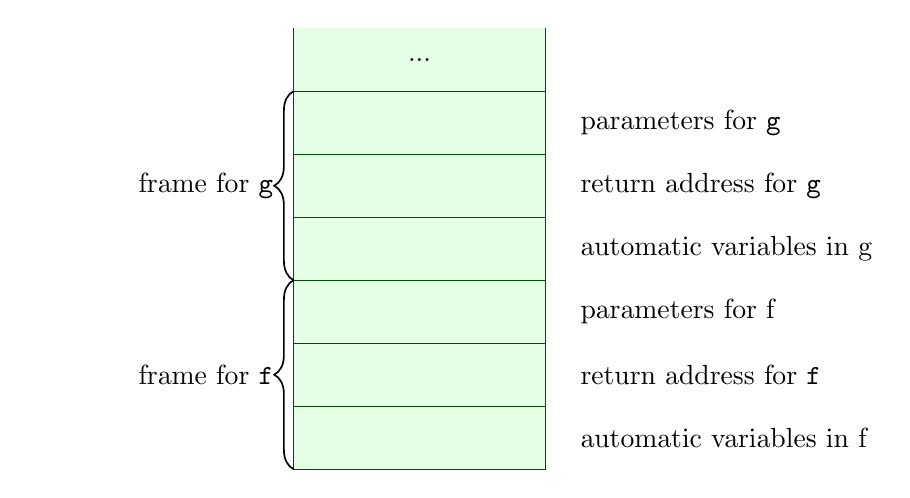
\begin{tikzpicture}[scale=.8]
  \stacktop{}
  \startframe
      \cell{}  
\cellcom{parameters for \texttt g} 
    \cell{}  
\cellcom{return address for \texttt g} 
      \cell{}        
    \cellcom{automatic variables in g}         
\finishframe{frame for \texttt g\ } 
  \startframe
  \cell{}  
    \cellcom{parameters for f} 
  \cell{}  
\cellcom{return address  for \texttt f} 
  \cell{}  
    \cellcom{automatic variables in f}
 \finishframe{frame for \texttt f\ } 
\end{tikzpicture}
There may be more in the frame, e.g. saved registers  
\end{frame}   


\begin{frame}[fragile]{Call stack: one frame per function \alert{call}}

%On most hardware, the stack grows towards smaller addresses.

Recursion example: fac(n) calls fac(n - 1) 
\\[2em]

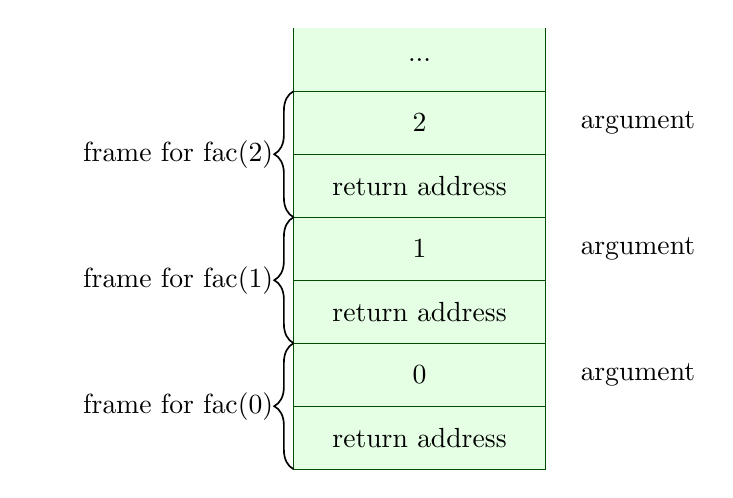
\begin{tikzpicture}[scale=.8]
  \stacktop{}
    \startframe
      \cell{2}  
    \cellcom{argument}
  \cell{return address}  
  \finishframe{frame for {fac(2)}} 
  \startframe
      \cell{1}  
    \cellcom{argument}
  \cell{return address}  
  \finishframe{frame for {fac(1)}} 
  \startframe
  \cell{0}  
    \cellcom{argument} 
  \cell{return address}  
 \finishframe{frame for fac(0)} 
\end{tikzpicture}

\end{frame}   


\section{Target architecture}

\begin{frame}{Target architecture}

We will only need a tiny subset of assembly.

Quite readable.

Instruction we will need:

mov push pop call ret jmp add mul test be

The call instruction pushes the current instruction pointer onto the stack as the return address

ret pops the return address from the stack and makes it the new instruction pointer

A nice target architecture should have lots of general-purpose registers with indexed addressing.

Like RISC, but x86 is getting there in the 64-bit architecture

\end{frame}

\begin{frame}{x86 in AT\&T syntax}

mov syntax is target last

\texttt{mov} x y is like y = x ;

Assembly generated by clang version 3.3

r prefix on registers means 64 bit register

movq etc: q suffix means quadword = 64 bits

\texttt{\%} register

\texttt{\$} constant

indexed addressing \texttt{-24(\%rbp)}

\end{frame}


\begin{frame}[fragile]{Clang function idiom}

\url{http://llvm.org/docs/LangRef.html#calling-conventions}

\begin{verbatim}
f:
	pushq	%rbp
	movq	%rsp, %rbp
    ... body of function f
	popq	%rbp
	ret
\end{verbatim}

parameters are passed in registers rdi, rsi

return value is passed in register rax
\end{frame}


\end{document}

